\documentclass{beamer}
\title{The Impact of Anthropogenic Forcing on ENSO Amplitude}
\author{Ben Goldman}
\date{\today}
\usepackage{natbib}
\usepackage{tikz}
\usetheme{metropolis}
\renewcommand{\bibsection}{}

% \begin{frame}{Example Frame With Text and Image}
%   \begin{columns}
%     \column{0.5\textwidth}
%     \begin{itemize}
%     \item Here we go...
%     \end{itemize}
%     \column{0.5\textwidth}
%     \begin{figure}
%       \centering
%       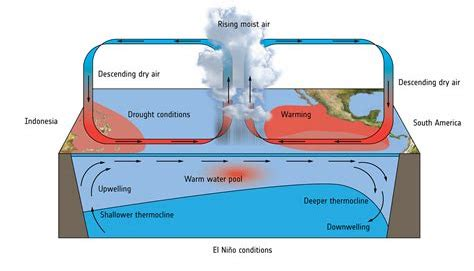
\includegraphics[width=\textwidth]{figures/example.jpg}
%       \caption{This is a very nice figure}
%       \label{fig:this}
%     \end{figure}
%   \end{columns}
% \end{frame}


\begin{document}

\maketitle

\section{Introduction}

\begin{frame}{Climate Change}

  \begin{columns}
    \column{0.5\textwidth}
    \begin{itemize}
    \item Here we go...
    \item \cite{bjerknes1969atmospheric}
    \end{itemize}
    \column{0.5\textwidth}
    \begin{figure}
      \centering
      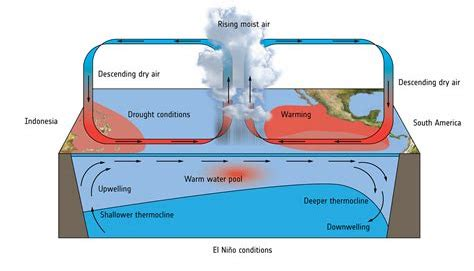
\includegraphics[width=\textwidth]{figures/example.jpg}
      \caption{This is a very nice figure}
      \label{fig:this}
    \end{figure}
  \end{columns}
\end{frame}

\begin{frame}{El Niño}

\end{frame}

\begin{frame}{Climate Simulation}

\end{frame}

\begin{frame}{ENSO in the Future}
  Problem: What effect does global warming have on ENSO? Can we expect ENSO to become stronger, weaker, or neither?
\end{frame}

\begin{frame}{Gap and Goal}

\end{frame}

\begin{frame}{Research Questions}

\end{frame}

\section{Data and Methods}

\begin{frame}{Ensembles: CESM1 and CESM2}

\end{frame}

\begin{frame}{Analysis Tools}
  \begin{columns}[t]
    \column{.33\textwidth}
    R:
    \begin{itemize}
    \item ncdf4
    \item zoo
    \item dplyr
    \item ggplot2
    \item WaveletComp
    \item reshape2
    \end{itemize}
    \column{.33\textwidth}
    Python:
    \begin{itemize}
    \item numpy
    \item pandas
    \item scipy
    \item matplotlib
    \item netCDF4
    \end{itemize}
    \column{.33\textwidth}
    Other:
    \begin{itemize}
    \item nco
    \end{itemize}
  \end{columns}

\end{frame}

\begin{frame}{Role of Mentor and Student}
  \begin{columns}[t]
    \column{.5\textwidth}
    Mentor:
    \begin{itemize}
    \item Suggest future methods
    \item Conduct parallel analysis to complement student work
    \item Provide raw precollected data
    \item Interpret data produced by student
    \item Review student writing
    \end{itemize}
    \column{.5\textwidth}
    Student:
    \begin{itemize}
    \item Analyze data on computer
    \item Produce graphics for analysis and publication
    \item Write documentation
    \item Suggest interpretations of data
    \end{itemize}
  \end{columns}

\end{frame}

\begin{frame}{Measuring ENSO}

\end{frame}

\begin{frame}{Measuring ENSO Intensity}

\end{frame}

\begin{frame}{Signal and Noise}

\end{frame}

\begin{frame}{ENSO is Becoming Stronger}

\end{frame}

\begin{frame}{It's not That Simple}

\end{frame}

\begin{frame}{Single Forcing Ensembles}

\end{frame}

\begin{frame}{Influence of Aerosols and Greenhouse Gasses}

\end{frame}

\begin{frame}{Correlation With Ocean Temperature}

\end{frame}

\begin{frame}{Stratification}

\end{frame}

\begin{frame}{Stratification in Other Ensembles}

\end{frame}

\section{Conclusion}

\begin{frame}{Conclusions}

\end{frame}

\begin{frame}{Discussion}

\end{frame}

\begin{frame}{Acknowledgments}

\end{frame}

\begin{frame}{References}
  \bibliographystyle{apalike}
  \bibliography{references.bib}
\end{frame}

\maketitle

\end{document}
